\documentclass[10pt,a4paper]{article}
\usepackage[margin=2.2cm]{geometry}
\usepackage{fontspec}
\usepackage{kotex}
\setmainfont{Apple SD Gothic Neo}
\setsansfont{Apple SD Gothic Neo}
\usepackage{amsmath,amssymb}
\usepackage{graphicx}
\usepackage{booktabs}
\usepackage{caption}
\usepackage[dvipsnames]{xcolor}
\usepackage[colorlinks=true,linkcolor=MidnightBlue,citecolor=MidnightBlue,
            urlcolor=MidnightBlue]{hyperref}
\usepackage{titlesec}
\titleformat{\section}{\large\bfseries}{\thesection}{0.6em}{}
\captionsetup{font=small,labelfont=bf}
\setlength{\parskip}{0.35em}
\setlength{\parindent}{0pt}

\usepackage{mdframed}
\newmdenv[linewidth=0.4pt,linecolor=gray!60,backgroundcolor=gray!5,
          innertopmargin=6pt,innerbottommargin=6pt,skipabove=8pt,skipbelow=8pt]{claimbox}
\newcommand{\claim}[2]{\begin{claimbox}\textbf{주장.} #1\par\smallskip
  \textcolor{gray!70}{\textbf{반증 조건.} #2}\end{claimbox}}

\title{\bfseries 얇은 장, 네 도메인\\[2pt]
\large 문패 셋($813 \cdot 814 \cdot 818$)이 닫혔다 --- 그리고 무리는 별 모양이다}
\author{월드모델 실험실 · 노트 $839$}
\date{2026-08-08}
\begin{document}\maketitle

\section{한 줄}

$838$ 의 `무리 확장 후보'가 판별 널을 통과했다(갈래 $2$ · 예측 $70\%$ 적중):
합성 판별력 `같다' $0$(파이프라인 유효) · 실측 $6$쌍 both-정규화 \textbf{같다
$3$ · 모른다 $3$ · 다르다 $0$} · 시간만 정규화 \textbf{$6/6$ 갈라짐}(`같다'는
진폭$+$시간 둘 다 제거 후만 --- 얇은 장 유지). \textbf{$4$-무리(게임 · 모바일 ·
세계애니 · 영화) 확정 · $813/814/818$ 문패 완결.}

\begin{figure}[t]\centering
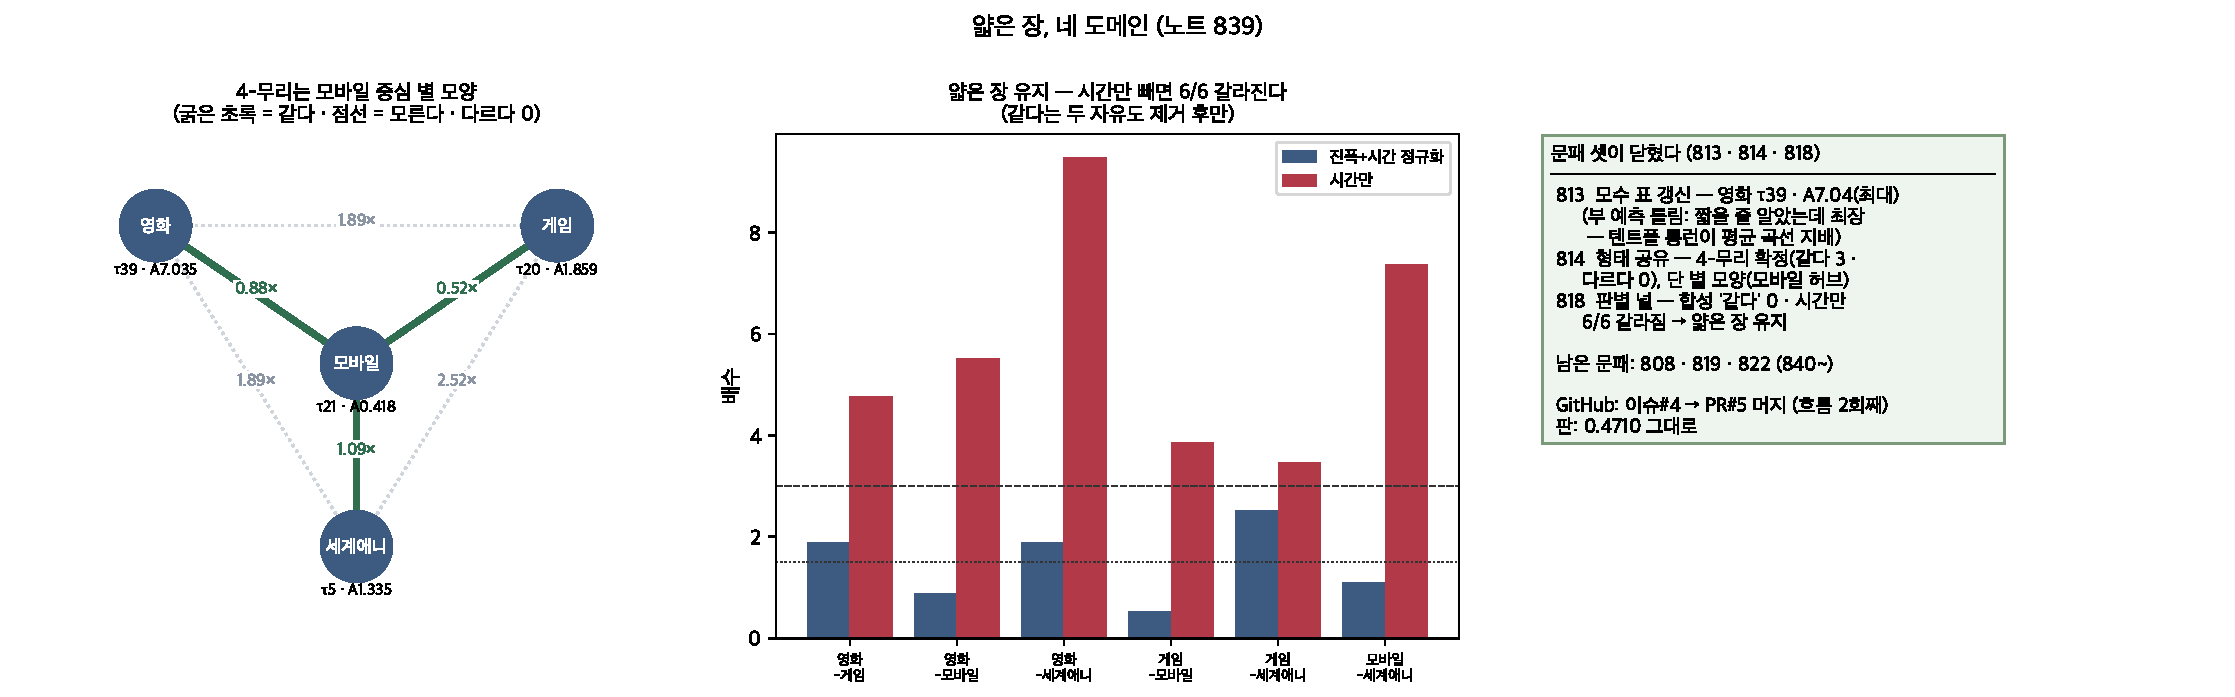
\includegraphics[width=0.99\textwidth]{figs/four.pdf}
\caption{왼쪽: 무리 그래프 --- 모바일 중심 별 모양. 가운데: 두 정규화 팔.
오른쪽: 문패 결산.}
\end{figure}

\section{별 모양, 그리고 텐트폴의 시간}

\claim{\textbf{`같다' $3$건이 전부 모바일을 포함한다} --- 영화-모바일
$0.88\times$ · 게임-모바일 $0.52\times$ · 모바일-세계애니 $1.09\times$, 비(非)모바일
쌍은 셋 다 모른다. 곡선 무리는 완전 그래프가 아니라 \textbf{모바일 허브의 별
모양}이다 --- 인수분해 가설(공유 형태 $\times$ 도메인 모수)의 다음 정밀화
재료. 모수 표($813$ 갱신): \textbf{영화 $\tau = 39$일 · 진폭 $7.04$(판 최대)}
· 게임 $20/1.86$ · 모바일 $21/0.42$ · 세계애니 $5/1.34$.}
{부 예측 채점의 정직: 영화 $\tau$ 가 위키 무리보다 \emph{짧을} 것($60\%$)이라
했는데 \textbf{최장}이다 --- 극장 소비는 개봉 주 집중이 아니라 q$85$ 문턱 위
모집단(텐트폴)의 롱런이 평균 곡선을 지배한다. 시간만 팔의 위키 $3$쌍
재현($80\%$)은 적중. 남은 문패: $808 \cdot 819 \cdot 822$($840{\sim}$).
GitHub 흐름(이슈 \#$4 \to$ PR \#$5$ 머지) $2$회째 완주. 판 $\rho$ $0.4710$
그대로.}

\end{document}
